\documentclass{ecnreport}

\stud{Master 1 CORO / Option Robotique}
\topic{Robot Operating System (2)}
\author{O. Kermorgant}

\begin{document}

\inserttitle{Robot Operating System}

\insertsubtitle{Lab 1: Packages, launch files,  parameters and topic remapping}

\section{Goals}

In this lab we will see the main tools to analyze nodes and topics.

\subsection{Using the terminals}

In ROS, a lot of commands have to be run from the terminal. Each terminal should be configured either to run ROS 1 things, or ROS 2 things.
A simple shortcut allows changing this:
\begin{bashcodelarge}
ros1ws  # type this to configure the terminal for ROS 1 (default)
ros2ws  # type this to configure the terminal for ROS 2 (has to be done manually)
\end{bashcodelarge}

You can change the default behavior by updating the ros1ws line of your \okttt{.bashrc} file.

Each time a package is compiled, the corresponding command (ros1ws / ros2ws) should be run in order to refresh the package list.

\subsection{Bring up Baxter}

Even if you have a real Baxter robot it can be a good idea to test the lab in simulation first.
In both cases, we want to have a RViz display, which is mandatory in simulation and quite handy on the real robot. RViz is run automatically in both cases.

\subsubsection{On the real robot}

Baxter is a ROS1-based robot. To work with ROS 2 we thus have to run a bridge that transforms all or some topics between ROS 1 and ROS 2.

A launch file is available in the \okttt{baxter_bridge} package to run both the bridge and RViz.

You have to connect to Baxter's ROSMASTER in the terminal where you run the bridge:
\begin{bashcodelarge}
 ros2ws
 source ~/ros/baxter.sh # so that your ROSMASTER is Baxter
 ros2 launch baxter_bridge baxter_bridge_launch.py
\end{bashcodelarge}

In you are in a lab on the real Baxter, remind the lab assistant to allow multiple publishers for this lab.
It can be done from a ROS 1 terminal:
\begin{bashcodelarge}
 ros1ws
 source ~/ros/baxter.sh # so that your ROSMASTER is Baxter
 rosparam set allow_multiple true
\end{bashcodelarge}

\subsubsection{In simulation (including virtual machine users)}

The Baxter simulator behaves as the actual Baxter from the ROS 2 side, only with a very limited part of the same topics and services. 

The \okttt{baxter_bridge} node should be run from a ROS 2 terminal:
\begin{bashcodelarge}
ros2ws
ros2 launch baxter_simple_sim sim_launch.py
\end{bashcodelarge}
The launch file also runs RViz.

\subsection{Initial state}

Whether in simulation or on the robot, Baxter is not moving and is waiting for commands on any arm.\\
A few in/out topics exist and can be listed through:
\begin{bashcodelarge}
rostopic list (ROS 1, if on the real robot)
ros2 topic list (ROS 2)
\end{bashcodelarge}

\subsection{Compiling the package}

The folder should be put in your ROS 2 workspace (\okttt{\~/ros2/src}). Compilation is done by calling colcon from the root of the workspace:
\begin{bashcodelarge}
 ros2ws
 cd ~/ros2
 colbuild --packages-select move_joint
\end{bashcodelarge}

\section{Running the control nodes}

A basic control GUI can be run with:

\begin{bashcodelarge}
 ros2 launch move_joint slider_launch.py
\end{bashcodelarge}
It runs a node that sends the slider value on a topic (here \okttt{setpoint}).\\

The Baxter robot has $2\times 7$ joints as shown in \Fig{baxter}, the names of which are listed in the table.
\begin{figure}[h]\centering
 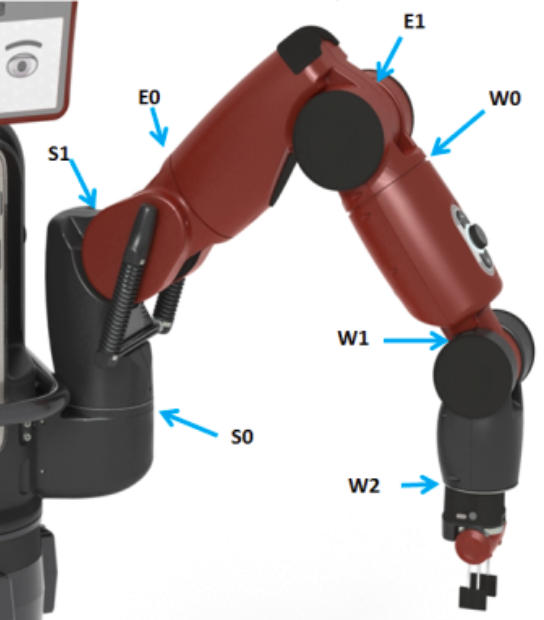
\includegraphics[width=.3\linewidth]{baxter} \\
  \begin{tabular}{|c|c|c|c|c|c|c|c|}
  \hline
  joints (\okttt{left_} \& \okttt{right_})& \okttt{s0} & \okttt{s1}& \okttt{e0} & \okttt{e1} & \okttt{w0} & \okttt{w1} & \okttt{w2} \\\hline
 \end{tabular}
 \caption{Baxter joints}
 \label{baxter}
\end{figure}

A special node called \okttt{move_joint} should be used to change the value published by the slider GUI, to the setpoint of a particular joint:
\begin{bashcodelarge}
 ros2 run move_joint move_joint
\end{bashcodelarge}

\subsection{Initial state of the control nodes}

Use \okttt{ros2 node} and \okttt{ros2 topic} to get the information on the nodes. There are currently two limitations:
\begin{itemize}
 \item The \okttt{move_joint} node needs a parameter to tell which joint it should be controlling
 \item The slider publishes on \okttt{setpoint} while the  \okttt{move_joint} node listens to \okttt{joint_setpoint}
\end{itemize}
Additionally, it would be nice to run the two nodes in the same lauch file.

\subsection{Regroup all nodes in the same launch file}

Open the \okttt{slider_launch.py} and add a line equivalent to calling \okttt{ros2 run move_joint move_joint}.\\
Then, add a parameter to tell which joint should be controlled:\\\okttt{parameters = \{'joint_name': 'right_e0'\}}\\

To run this launch file, you can go to its folder and type \okttt{ros2 launch ./slider_launch.py}.\\
Display the graph (\okttt{rqt_graph}) to detect that the slider node and \okttt{move_joint} do not communicate, because they do not use the same topics.

\subsection{Remapping}

In this section we will remap the topic name of \okttt{move_joint} such that is uses \okttt{setpoint} instead of \okttt{joint_setpoint}.\\

Modify the launch file by adding this argument to the \okttt{move_joint} node:

\begin{pythoncodelarge}
remappings = {'joint_setpoint': 'setpoint'}.items()
\end{pythoncodelarge}
Run the launch file again and you should be able to control the chosen joint.

\section{Playing with launch files}

\subsection{Argument for joint name}

Now that a launch file exists to control 1 joint from a slider, we will change the hard-coded joint name to an argument:
\begin{pythoncodelarge}
sl.declare_arg('name', 'right_e0')
\end{pythoncodelarge}
This syntax tells the launch file that is now has a \okttt{name} argument, with default value \okttt{'right_e0'}.\\

Change the hard-coded value to the argument one \okttt{sl.arg('right_e0')} and check that the behavior is the same\\

Also, you can rename the slider GUI by giving an additional argument:
\begin{pythoncodelarge}
sl.node('slider_publisher', 'slider_publisher', name=sl.arg('name'), ...)
\end{pythoncodelarge}

Then, run the launch file with another name, for instance:\\ \okttt{ros2 launch ./slider_launch.py name:=left_e0}\\
On another terminal, try to run the same launch file for another joint. What happens?\\



\subsection{Including launch files in other launch files}

In this last section we will write a new launch file that will include the previous one, for various joint names. In order to avoid node / topic duplicates, each nodes relative to a specific joint will be in their own namespace. 

The syntax to include a launch file in another one is as follow:
\begin{pythoncodelarge}
sl.include('move_joint', 'slider_launch.py', launch_arguments = [('name', 'right_e0')])
\end{pythoncodelarge}

It should be called from a namespace block, with this syntax:
\begin{pythoncodelarge}
with sl.group(ns = 'right_e0'):
  sl.include('move_joint', 'slider_launch.py', launch_arguments = [('name', 'right_e0')])
\end{pythoncodelarge}

Check that the behavior is similar to the previous one. Then, write a for loop to run this code for many joint names:
\begin{pythoncodelarge}
joints = ('right_e0', 'right_e1', ...)
for joint in joints:
    with sl.group(ns = joint):
        sl.include(...)
\end{pythoncodelarge}



\end{document}
